\documentclass[10pt,letterpaper,landscape]{article}
\usepackage[utf8]{inputenc}
\usepackage[T1]{fontenc}
\usepackage[letterpaper,landscape,margin=0in]{geometry}
\usepackage{graphicx}
\usepackage{microtype}
\usepackage{multicol}
\usepackage{xcolor}
\usepackage[absolute,overlay]{textpos}
\usepackage{tikz}
\setlength{\parindent}{0pt}
\setlength{\parskip}{0.08em}
\pagestyle{empty}
\sloppy

\setlength{\TPHorizModule}{1in}
\setlength{\TPVertModule}{1in}
\textblockorigin{0in}{0in}

\newenvironment{acpanel}[2]{%
  \begin{textblock*}{5.06in}(#1,#2)%
    \begin{minipage}[t][8.06in][t]{5.06in}%
      \raggedright%
}{%
    \end{minipage}%
  \end{textblock*}%
}

\newcommand{\foldline}{%
  \begin{textblock*}{0.01in}(5.5in,0in)
    {\color{black!35}\rule{0.6pt}{8.5in}}
  \end{textblock*}
}

\newcommand{\glitchtitle}[1]{%
\begin{tikzpicture}[baseline=(main.base)]
  \node[inner sep=0pt,outer sep=0pt,text=cyan!65] at (-1.5pt,1.0pt) {\fontsize{54}{56}\selectfont\bfseries #1};
  \node[inner sep=0pt,outer sep=0pt,text=magenta!60] at (1.5pt,-1.0pt) {\fontsize{54}{56}\selectfont\bfseries #1};
  \node (main) [inner sep=0pt,outer sep=0pt,text=black] at (0,0) {\fontsize{54}{56}\selectfont\bfseries #1};
\end{tikzpicture}%
}

\newcommand{\infoblock}[2]{%
\noindent\colorbox{black!5}{%
\parbox{\dimexpr\linewidth-2\fboxsep\relax}{%
{\fontsize{8.45}{9.35}\selectfont\textbf{#1}}\\[-0.1em]
{\fontsize{7.7}{8.55}\selectfont #2}
}}\vspace{0.05in}
}

\newcommand{\ritualcard}[3]{%
\noindent\colorbox{black!4}{%
\parbox{\dimexpr\linewidth-2\fboxsep\relax}{%
\vspace{0.02in}
\begin{minipage}[t]{0.27\linewidth}
\includegraphics[width=\linewidth,height=0.84in,keepaspectratio]{#3}
\end{minipage}\hfill
\begin{minipage}[t]{0.68\linewidth}
{\fontsize{10.9}{11.8}\selectfont\textbf{#1}}\\[-0.1em]
{\fontsize{9.1}{10.0}\selectfont #2}
\end{minipage}
\vspace{0.01in}
}}
\vspace{0.08in}
}

\newcommand{\seqstrip}[3]{%
\begin{tikzpicture}
\begin{scope}
\path[clip] (0,0) rectangle (\linewidth,1.52in);
\node[anchor=center,inner sep=0pt] at (0.5\linewidth,0.76in) {\includegraphics[width=\linewidth]{#3}};
\end{scope}
\fill[black,opacity=0.22] (0,0) rectangle (\linewidth,1.52in);
\node[anchor=north west,text=white] at (0.09in,1.43in) {\fontsize{27}{28}\selectfont\bfseries #1};
\node[anchor=south west,text=white] at (0.10in,0.08in) {\fontsize{13.5}{14.4}\selectfont #2};
\end{tikzpicture}\vspace{0.03in}
}

\newcommand{\biochip}[2]{%
\begingroup
\setlength{\fboxsep}{1.5pt}%
\noindent\colorbox{black!4}{%
\parbox{\dimexpr\linewidth-2\fboxsep\relax}{%
{\fontsize{6.2}{6.8}\selectfont\textbf{#1}}\\[-0.14em]
{\fontsize{5.1}{5.75}\selectfont #2}
}}\vspace{0.038in}
\endgroup
}

\newcommand{\biorow}[2]{\biochip{#1}{#2}}
\newcommand{\biomini}[2]{\biochip{#1}{#2}}

\begin{document}
\null

% OUTSIDE PAGE: left = back, right = front cover
\foldline

\begin{acpanel}{0.22in}{0.22in}
\begin{center}
{\fontsize{16}{17}\selectfont\textbf{Dis-Order}}\\[-0.18em]
{\fontsize{8.7}{9.6}\selectfont bios}
\end{center}
\vspace{0.08in}
\hrule
\vspace{0.05in}

\biorow{Mamie Green}{is a choreographer and the director of VOLTA, an interdisciplinary performance project that fuses physicality, theatricality, and multidisciplinary approaches to performance. Named in Fjord Review's ``Best of Dance 2023'' and Bachtrack's ``Young Choreographers to Watch,'' Green's work has been presented across the US, Europe, and the UK at the MAXXI National Museum, Jeffrey Deitch, Ace Hotel Brooklyn, MAK Center at the Schindler House, New Hollywood Theater, and Skirball Cultural Center with upcoming presentations at the Guggenheim Museum in Bilbao Spain and the Foster Theater in Portland, Oregon in 2026. Green holds a BFA from Mason Gross School of the Arts.}
\biorow{Freak Nature Puppets}{is an artist collective from Los Angeles, CA. Their work channels dreamlike narratives through giant puppetry, leading to unexpected and playful conclusions. Freak Nature's theatrical work is inspired by the avant-garde progressive puppetry of Bread and Puppet Theater, the oddball physical theater of Mummenshanz, and the anarchist children's entertainment of Pee-Wee Herman. Freak Nature's past collaborators \& co-presenters include Dead \& Company, the Bob Baker Marionette Theater, Eric Andre, KCRW, Poncili Creacion, David Zwirner Gallery, and Childish Gambino.}
\biorow{Rebecca Schultz}{writes fiction and criticism. Her work has appeared in the Los Angeles Review of Books, BOMB, Full-Stop, and the Santa Monica Review, where it was nominated for a Pushcart Prize. She teaches fiction and poetry at UC Irvine.}
\biorow{Patrick Shiroishi}{is a Japanese-American multi-instrumentalist, composer \& poet based in Los Angeles. Over the last decade he has established himself as one of the premier improvising musicians in the city, playing solo \& in numerous collaborative projects. He has presented work \& performed at the Museum of Contemporary Art, the Metropolitan Museum of Art, the Broad Museum, The Getty, commissioned by the LA Philharmonic \& has toured around the world in various solo \& band configurations including The Armed \& contemporary classical ensemble Wild Up.}
\biorow{Dylan Fujioka}{is a Japanese American multi-instrumentalist \& composer born and raised in Los Angeles, CA. He is most known for his drumming/recording \& performances in bands across multiple genres and collaborations. He also composes for film and television. His multicultural upbringing has directly shaped and influenced his style and sound.}
\biorow{Sophie Becker}{is a New York-based ventriloquist and actor working at the intersection of ventriloquism, theater, and experimental comedy. With a cast of recurring characters, including her dummy, Ronnie, Sophie has performed at MoMA PS1, De Studio (Belgium), the Marriott Marquis in Times Square, the Rockaway Film Festival, Jean's Lafayette, Art Omi, and NADA Miami, among others.}
\biorow{Ari Salka}{is a Los Angeles-based artist whose practice spans painting, drawing, and poetry. He received a BFA from SAIC (2016) and an MFA in Painting from UCLA (2019). Salka was awarded the Yale Norfolk Summer School of Art's Ellen Battell Stoeckel Fellowship in Norfolk, CT (2015). Salka has lectured as a visiting artist at UCLA, Chapman University, and Bennington College. Salka's work is in the permanent collections of the John M. Flaxman Library, LACA, UCLA Arts Library, and the ROSA KWIR Archive. His artist book is currently available for purchase at MOCA, and he looks forward to an upcoming solo museum exhibition at XELA Art in 2027.}
\biorow{Roxanne Steinberg}{is a dancer and choreographer. She founded Body Weather in Los Angeles in 1988 based on the Japanese paradigm for training. Her solos have been presented at the REDCAT, Dance Conversations at the Flea, NY, the Basilica in Hudson NY, Zebulon LA and in Flower of the Season, the dance series she co-directs at the Electric Lodge. She has led workshops at Cal Arts, UCLA and choreographed works for Cal State LA and Body Vox in Portland.}
\end{acpanel}

\begin{textblock*}{5.5in}(5.5in,0in)
\begin{tikzpicture}
\path[clip] (0,0) rectangle (5.5in,8.5in);
\node[anchor=center,inner sep=0pt,opacity=0.26] at (2.75in,4.25in) {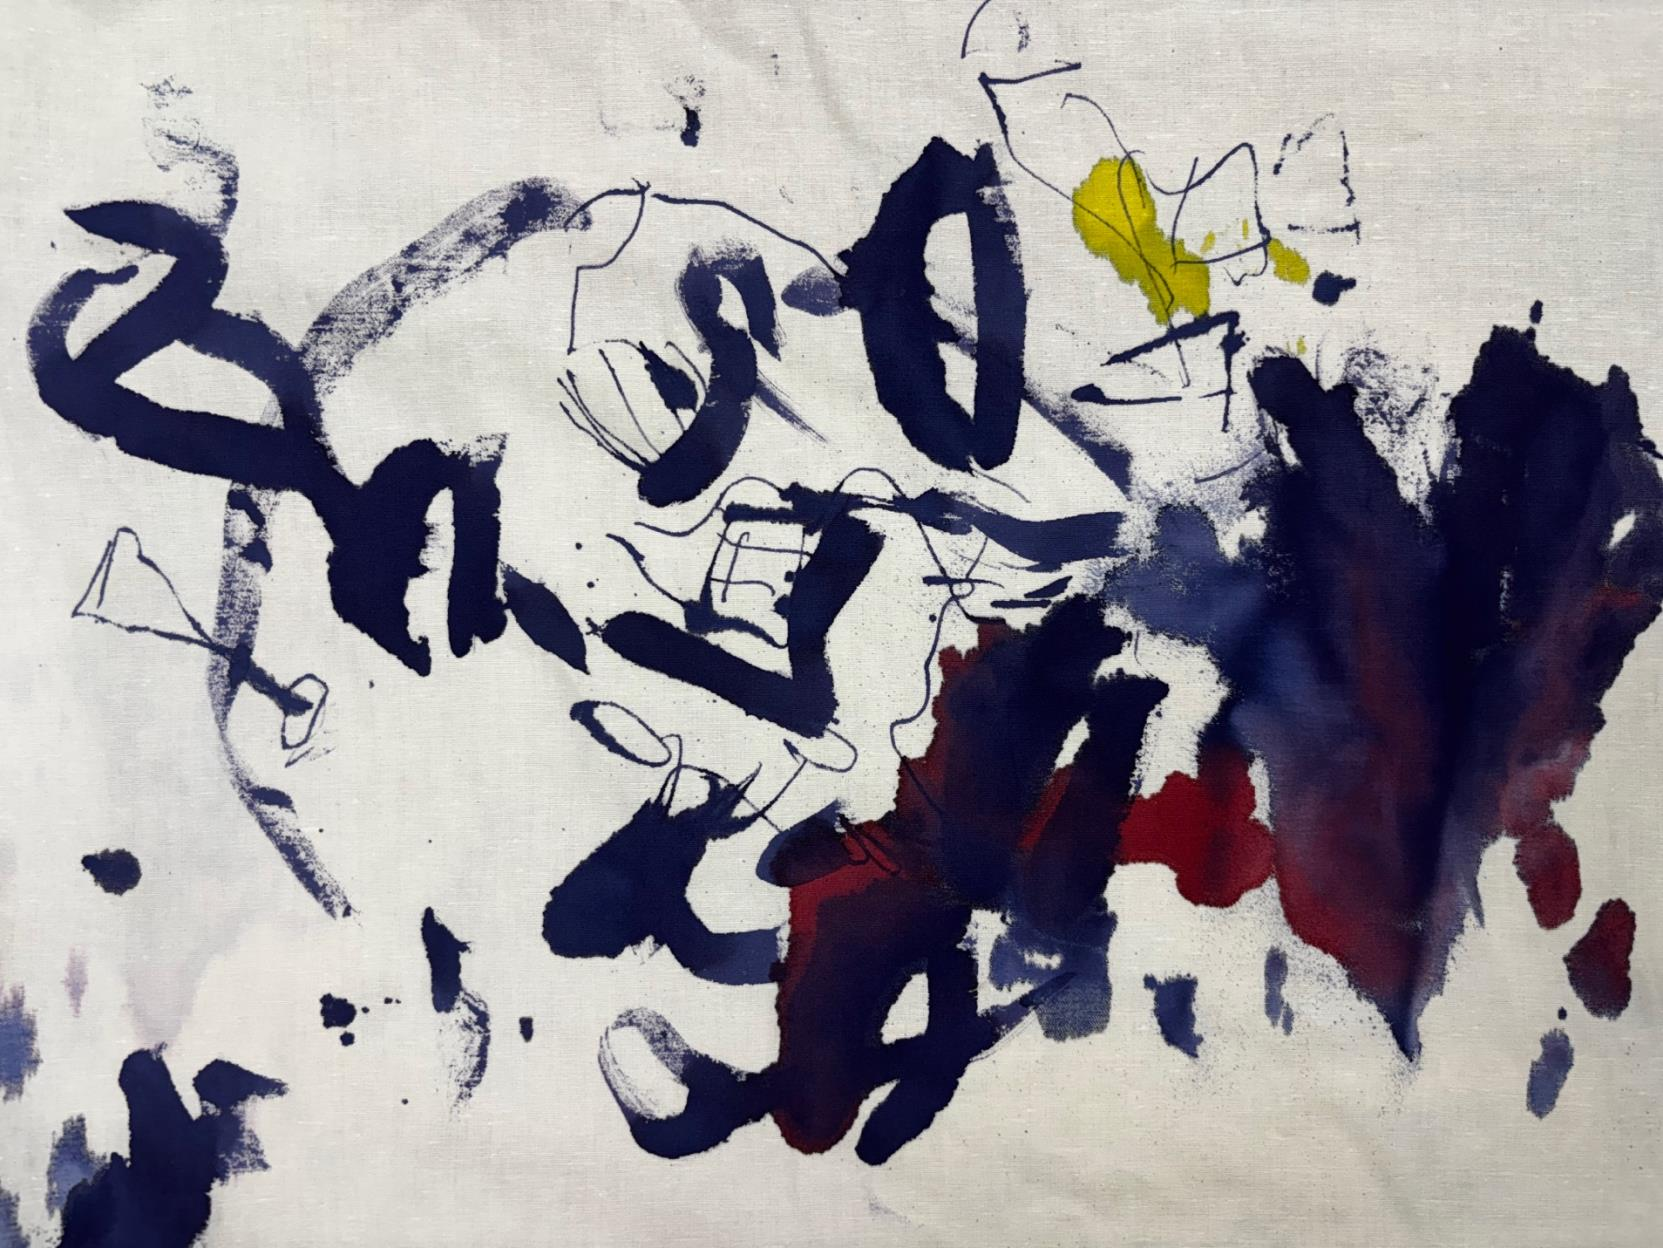
\includegraphics[height=8.5in]{images-v2/cover.jpg}};
\end{tikzpicture}
\end{textblock*}

\begin{textblock*}{5.5in}(5.5in,0in)
\begin{minipage}[t][8.5in][c]{5.5in}
\begin{center}
  \glitchtitle{Dis-Order}\\[0.4em]
  {\fontsize{18}{20}\selectfont welcome,}\\[-0.03em]
  {\fontsize{18}{20}\selectfont we've been waiting for you}
\end{center}
\end{minipage}
\end{textblock*}

\newpage
\null

% INSIDE PAGE: left = ritual image sequence, right = body copy + credits
\foldline

\begin{acpanel}{0.22in}{0.22in}
\seqstrip{I.}{begin with fire}{images-v2/i-candles.jpg}
\seqstrip{II.}{wicked child bacchanal}{images-v2/ii-donkey.jpg}
\seqstrip{III.}{total darkness}{images-v2/iii-egg.jpg}
\seqstrip{IV.}{lovers' pastoral}{images-v2/iv-pastoral.jpg}
\seqstrip{V.}{death of the first born}{images-v2/v-daughter.jpg}
\end{acpanel}

\begin{acpanel}{5.72in}{0.22in}
{\fontsize{11.2}{12.3}\selectfont\textbf{Dis-order}}\\[0.03in]
{\fontsize{8.7}{9.55}\selectfont
Dis-order is a performance, communal ritual, and a family drama that asks what forces move through us when we enact an ancient spring rite, and what is left unspoken when we gather around the table.

Staged a la Judy Chicago's \textit{The Dinner Party}, the piece references the Passover seder, Greek mythology, and Pina Bausch's \textit{Rite of Spring} to examine the performance of ritual and the rigidity of roles and stories within families, communities, and institutions.
}

\vspace{0.08in}
\infoblock{Performed by}{Sophie Becker, Tim Allen, Roxanne Steinberg, Ryley Polak, Anaya Gonzales, Nico Fife, and Abby Sage.}

\infoblock{Creative Team}{Choreographed and directed by Mamie Green. Concept by Mamie Green and Rebecca Schultz. Puppets by Freak Nature Puppets and Abby Sage. Original live score by Patrick Shiroishi and Dylan Fujioka. Script by Rebecca Schultz. Set design by Ari Salka. Dramaturgy by Livia Reiner.}

\infoblock{Thanks}{Thank you to the Skirball Cultural Center, Community Engagement Grants, Oracle Egg BROILER Residency, and Reboot for supporting this project.}
\vspace{0.02in}

\biomini{Ryley Polak}{is a dancer and teacher based in Los Angeles, California where he received his BFA in commercial dance from Hussian College. Ryley was signed by the Movement Talent Agency which represents him as both a Dancer and Educator. Throughout his professional career he has worked on sets of commercials, movies, music videos, and TV shows such as A24's ``Dick's: The Musical'', ``VROOM'' SuperBowl commercial, and Anna Margo's ``Bad Friend'' music video. Ryley has been a performer with Mike Tyus, Jaclyn Royal, Mandy Moore, and many others and has performed internationally with Royal Flux and Volta Collective in Italy, Canada, London, Cyprus, and more.}
\biomini{Anaya Gonzalez}{is a dancer that enjoys promoting emotional experiences for others through movement and is deeply determined in the pursuit of crafting and cultivating art. They have studied at the University of North Carolina School of the Arts, studying ballet \& the following contemporary techniques: Limon, Cunningham, Alexander, floorwork and has performed pieces by Darrel Moultrie, Rena Butler, Jose Limon, and Trey McIntyre. During her professional career she was recently a full time BODYTRAFFIC company dancer performing works by Micaela Taylor, Matthew Neenan, Juel D. Lane, and Trey Mcintyre.}
\biomini{Nico Fife}{is an actor, writer, puppeteer, director, and strong mover from Long Beach, California. Nico received a BA in Theater from USC, and is currently an Associate Company Member at The Actors' Gang Theater Company in Culver City. Nico is an active practitioner and teacher of Viewpoints, especially working with youth and with formerly incarcerated artists. Nico has recently performed in Children of The Winter Kingdom (Crow, Emperor Weasel, Ensemble) with The Actors' Gang, in Clown Pit Revolution (Sasha Faguette), and various comedy shows throughout the city. Thank you to Mamie, to Sater \& Freak Nature Puppets, and to the entire cast and crew for having me on this journey!}
\biomini{Tim Griffin Allan}{is a New York based actor thrilled to be here and briefly escaping the frigid East Coast winter. He has recently performed in plays at Pioneer Works, Abrons Arts Center, and Studio 17. On screen, he has appeared in films and television shows for A24, HBO, MUBI, and CBS. Allan is also a member of a rival puppet troupe PussyPaws Puppetry, though he agreed to a temporary puppet truce, hiding the felt knives in order to collaborate with Freak Nature, Mamie Green, and this dangerously talented cast.}
\biomini{Abby Sage}{is a singer, songwriter, and multidisciplinary artist whose work blends storytelling with a cinematic sense of atmosphere. Known for her haunting vocals and emotionally vivid songwriting, Sage's music explores themes of vulnerability, transformation, and memory, often drawing listeners into deeply personal yet expansive sonic worlds. Beyond music, Sage's creative practice extends into visual and performance art. She builds and designs handcrafted puppets, using them as expressive characters that blur the boundaries between object, performer, and storyteller. Her puppetry explores movement, symbolism, and the emotional language of gesture.}
\biomini{The Skirball Cultural Center}{is a place of meeting guided by the Jewish tradition of welcoming the stranger and inspired by the American democratic ideals of freedom and equality. We welcome people of all communities and generations to participate in cultural experiences that celebrate discovery and hope, foster human connections, and call upon us to help build a more just society.}
\end{acpanel}

\end{document}
